\documentclass[oneside,11pt,book]{book}

\usepackage{amsmath}
\usepackage{amsfonts}
\usepackage{amssymb}
\usepackage{graphicx}
\usepackage{auto-pst-pdf}%for converting pstricks diagrams for compilation in pdflatex
\usepackage{pst-optexp} %for optics diagrams using pstricks
\usepackage{wasysym} %for the sun symbol used for light source
%\usepackage{subfig}
%\usepackage[para,symbol*]{footmisc}
\usepackage{tikz}
\usepackage{color}
\usepackage{subcaption}


\begin{document}

\chapter{Experimental Methodology}
\section{Sample Fabrication}
\subsection{Electron Beam Lithography}

All electron beam lithography steps are performed in an ISO class 6 cleanroom. This minimises the risk of small particle contamination and unwanted organic residues being introduced to the samples.

An Si wafer is prepared as a master substrate.  Any large-particle dust is removed from the wafer surface using pressurised Nitrogen gas. The wafer surface is then spin-coated in a 600 nm thick protective layer of Poly(methyl methacrylate) (PMMA). The typical protective polymer used was PMMA 950K A6, spun at 2000 RPM for 40 seconds to produce the 600 nm layer. 
The wafer was then diced into 1 mm$^2$ chips which would be used as the  grating master substrates. The protective resist layer protects the chip surface from the Si dust that the dicing process produces. This layer, and the accompanying contamination, is removed by inverting the chips in  100 ml of warm Acetone for 10 minutes. After removing the protective resist, the chips are placed into a fresh solution of boiling Acetone ($80^\circ$C) for 1 hour, and then sonicated in 100 ml of Isopropanol for 1 hour. The substrates may occasionally splinter during sonication, (in doing so introducing unwanted Si dust to the solution), these chips are discarded. After 1 hour of sonication , the chips are removed from the isopropanol and dried using pressurised Nitrogen gas.
The clean wafer chips are then inspected under dark-field optical microscopy to ensure the surface is optically clean. If not, the cleaning process is repeated.

The electron resist is then added to the surface. The resist used in all grating fabrications included here is PMMA 950K A4. This is a positive electron-resist, whereby exposure of the resist to the electron beam causes de-cross linking of the polymer chain, allowing the removal of the exposed resist with developer. The chip is placed in a motorised spincoater, and 3-4 drops of PMMA is introduced to the surface using a new, clean glass pipette. The chip and resist is spun at 4500 RPM for 40 seconds to leave a 180 nm thick layer of resist on the surface. The substrate is then baked at 165$^\circ$C for 10 minutes on a hot-plate. This baking raises the resist temperature above the glass transition temperature, forming ideally a single crystal of PMMA across the substrate. The heat also causes the evaporation of any remaining solvent (Anisol), improving substrate adhesion. 

The substrate is then loaded into the electron lithography system and the grating pattern is exposed. The system used is a nB4 Electron Beam Lithography system (NanoBeam Limited) and exposures are performed with a beam current of 2 nA and a beam accelerating voltage of 80 keV. The exposure dose ranged between 400-600 $\mu$C cm$^{-2}$, depending on the grating. Initially, the grating pattern was exposed four times at different locations on one substrate, each grating using a different test dose. The final samples produced from these test areas are examined under scanning electron microscopy and the SPP response is measured using the optical techniques listed in section \ref{}, in order to determine the best electron dose to use for each particular grating. Future exposures of these gratings, where the dose had been previously determined, are limited to one grating per chip. 

The write field size, (the region exposed before the substrate needs to be moved) was 100 $\mu$m, to minimise the effect of height variation across the substrate.
The nB4 electron beam system has a theoretical beam size of 2.3 nm at 100 keV, and the stitching error between write-fields is on the order of 20 nm. This stitching error introduces an extremely weak long-pitch periodicity to the samples, on the order of the write field size. The weak diffractive properties from these stitching errors are not found to inhibit the optical efficiencies of the gratings, and are not observed experimentally.

The exposed sample then requires development to remove the de-cross-linked polymer and provide us with a polymer etching mask for the Si. The developer used is a 15:5:1 solution of IPA:meythl-whatever:methyl ethyl keytone. A small endothermic reaction occurs when this solution is first mixed, so to ensure development times remain consistent between processes the developer must be allowed to return to room temperature before use. 
The exposed chip is submerged in the solution for 1 minute, followed immediately by a further 1 minute in a beaker of IPA. When transferring the sample between the developer and the IPA, it is advisable to maintain a small amount of the developer in a droplet on the sample surface, to prevent premature exposure to the air. After the 1 minute in IPA, the sample is removed and blow-dried with Nitrogen gas. At this point the diffraction properties of the sample will be apparent, and illumination with an appropriate wavelength laser allows an estimation/check of the grating's periodicity and orientation.

At this stage, the grating pattern has been transferred to the resist and successfully developed. The sample consists of a coating of un-exposed PMMA layer, in which a 180 nm deep pattern has been developed. This polymer grating sits on a Si substrate. The pattern is now transferred to the Si chip by means of reactive ion etching (RIE), using the PMMA as a polymer mask. 
The reactive ion etching gas used is an oxygen, CHF mix,  with x cc O$_2$ y cc CHF$_3$ etc etc. This gives an etch rate into the Si of approximately 29 nm min$^{-1}$
We have found that the selectivity of Si to PMMA etching is sufficient for a 180 nm thick layer of PMMA to be a suitable etching mask for depths of up to 80 nm etched into the Si substrate. After RIE, any excess resist is removed by boiling the sample in acetone and sonication in IPA. This leaves a master grating pattern in a Si substrate.

For 'crossed' bigratings, where a second periodicity runs along the grating surface at an angle to the first periodicity, this process is repeated, with a previously fabricated Si master grating used in place of the flat Si substrate.
 
\subsection{Thermal Evaporation} 
 Evap silver (specifics)
clean glass substrate. acetone cotton buds, IPA drag-clean.
\subsection{Template Stripping}
apply Norland 60 (or 65) and cure for 20 minutes
 use a razor blade to remove master, leaving behind patterned silver.    
\subsection{Polymer replication}

\section{Angle scans}
\subsection{Monochromator}
\begin{figure}
\centering \begin{pspicture}[](11,6)

\pnode(0,3){S1}
\pnode(0,2){M1}
\pnode(1,3){Monoc}
\pnode(2,4){M2}
\pnode(3,2){M3}
\pnode(2,3){M4}
\pnode(4,3){P1}
\pnode(5,3){Chopper}
\pnode(6,3){Pol}
\pnode(7,3){L1}
\pnode(8,3){BS}
\pnode(8,4){D1}
\pnode(10,3){Grating}
\pnode(9,5){D2}

\mirror[mirrorradius=1.1,mirrortype=extended](S1)(M1)(Monoc){M1}
\optbox[innerlabel,allowbeaminside=false](M1)(M2){MC}
\mirror[mirrorradius=1.87,mirrortype=extended](Monoc)(M2)(M3){M2}
\mirror[mirrorradius=0.9,mirrortype=extended](M2)(M3)(M4){M3}
\mirror[labelangle=90,mirrortype=extended,mirrorwidth=0.3](M3)(M4)(L1){M4}
\pinhole[compname=pinhole,phwidth=0.1,innerheight=0.18,labelangle=180, compshift=0.05](M4)(Chopper){P}
\optbox[compname=chopper,optboxwidth=0.4,compshift=0.05](M4)(Pol){C}
\optplate[compname=pol,compshift=0.05](Chopper)(L1){Pol}
\lens[n=1.2,compname=L1](Pol)(BS){L}
\beamsplitter[compname=BS,bsstyle=plate,labelangle=-90](L1)(BS)(D1){BS}
\optdetector[compname=D1](BS)(D1){D1}
\optgrating[compname=grating,compshift=0.05](BS)(Grating)(D2){Sample}
\optdetector[compname=D2](Grating)(D2){D2}
\optplate[compname=pol2](Grating)(D2){Pol}
\rput(S1){\Large{\sun}}
\rput(10.6,3){\Large{$\circlearrowright$}}

\addtopsstyle{Beam}{fillstyle=solid, fillcolor=green,opacity=0.05,linestyle}
\drawwidebeam[beamdiv=14,ArrowInside=->,arrowscale=1.3](S1){1}{2}{3}{4}{5}{6}{7}{L1}{grating}{D2}
\drawwidebeam[beamdiv=14,ArrowInside=->,arrowscale=1](S1){1}{2}{3}{4}{5}{6}{7}{L1}{BS}{D1}

\addtopsstyle{Beam}{fillstyle=solid, fillcolor=blue,opacity=0.05,linestyle}
\drawwidebeam[beamdiv=14,ArrowInside=->,arrowscale=2,linecolor=blue](S1){1}{2}


\end{pspicture}
\caption{The monochromator \label{fig:monochromator}}
\end{figure}
To record the optical response of the diffraction gratings as a function of both incident wavelength, $\lambda_0$, and polar angle, $\theta$, a typical rotational stage/monochromator system is used. A schematic of the equipment is shown in figure \ref{fig:monochromator}. The incident wavelength is selected by directing a white light source through the monochromator via the focussing mirror, M1. Using an internal metallic diffraction grating and an output slit, the monochromator outputs a beam of almost monchromatic light with a spectral width of $\lambda_0\pm0.25$ nm, with a selectable wavelength range between 400 to 850 nm. This light is then collimated by a pair of mirrors, labelled M2 and M3 in figure \ref{fig:monchromator}, and directed down the primary optical axis by a plane mirror located at M4. The light is then spatially filtered by a 0.5 mm pinhole (P) and passed through a optical chopper (C) operating at approximately 1.3 KHz. The chopper's operating frequency is passed to a pair of phase-sensitive detectors and is used as the triggering frequency for the signals obtained from the photomultiplier tubes.
The beam is then passed through a linear polariser (Pol) with which the polarisation dependence of the optical response may be investigated.

For small-area samples, such as diffraction gratings fabricated using EBL, the grating area may be as small as 2 mm$^2$. In order to ensure the entire optical field impinges the grating, and not the surrounding material, the beam is focussed with a lens, L, with a focal length of 0.5 m. The distance between the pinhole, P, and the lens, L, is approximately 1 m, approximating to a collimated far-field image with a radius of 0.5 mm, which is reproduced at the lenses focal point. For smaller beam-spot areas, a smaller pinhole may be used, at the cost of detectable light intensity. 

A small fraction of the light is directed to a reference detector, D1 via a plane-glass beam splitter, BS. This reference signal allows for the normalization of the time-dependance of the white-light source intensity, which may vary over time. The transmitted beam continues along the primary optical axis and hits the sample positioned precisely on a robotic rotational stage, such that the sample position is central to the rotational axis and also at the focal position of lens L. The robotic table, controlled via computer, sets the polar angle, $\theta$ of the sample, with the spectral reflectivity detector, D2, mounted so that it moves a corresponding distance of $2\theta$.

The spectrally reflected light is collected by the detector D2 after passing though a second linear polariser. Both detectors, D1 and D2, are photomultipler tubes whose output current varies linearly with incident light intensity. The signal from the dectros is passed to a set of phase sensnsitve detector which, together with the chopper triggering signal, extracts the reference and reflectivity measurement and passes it to the computerized recording software via an analogue interface card.

\subsection{HeNe kit}
\begin{figure}
\centering \begin{pspicture}[](9,3)

\pnode(1,1){S}
\pnode(2,1){C}
\pnode(3,1){ND}
\pnode(4,1){Pol}
\pnode(5,1){BS}
\pnode(9,1){Grating}
\pnode(8,2){D2}
\pnode(5,2){D1}

\optbox[position=start,innerlabel, allowbeaminside=false,compname=laser](S)(C){HeNe}
\optbox[compname=chopper,optboxwidth=0.4](S)(ND){C}
\optplate(C)(Pol){ND}
\optplate(ND)(BS){Pol}
\lens[optional](BS)(Grating){L}
\beamsplitter[compname=BS,bsstyle=plate,labelangle=-90](Pol)(BS)(D1){BS}
\optgrating[compname=grating,labelangle=-90](BS)(Grating)(D2){Sample}
\optdetector[compname=D2,dettype=diode](Grating)(D2){D2}
\optdetector[compname=D1,dettype=diode](BS)(D1){D1}

\addtopsstyle{Beam}{fillstyle=solid, fillcolor=red,opacity=0.35,linestyle}
\drawwidebeam[beamwidth=0.1,ArrowInside=->,arrowscale=1.3,linecolor=red](S){grating}{D2}
\drawwidebeam[beamwidth=0.1,ArrowInside=->,arrowscale=1,linecolor=red](S){BS}{D1}
\rput(9.5,0.8){\Large{$\circlearrowright$}}
\end{pspicture}
\caption{The angle scan kit\label{fig:HeNe}}
\end{figure}
A similar set-up is used for acquiring angle dependant reflectivity of samples at a single wavelength. In this setup, shown in figure \ref{fig:HeNe}, a HeNe laser ($\lambda_0 = 632.8$ nm) is passed through an optical chopper, C, a neutral density filter, ND, and a polariser before a beamsplitter (BS) directs a small fraction of the beam to a reference detector. The beam transmitted through the beam splitter continues along the optical axis and is passed through an optional lens before impinging the sample placed, again, at the center of rotation of a robotic table. The detectors used are photo-diodes, whose voltage output is linearly dependant with respect to the incident intensity of light. The signal from the detectors are passed to a set of phase sensitive detectors, and the signal extracted, as before, using the mechanical chopper as a triggering reference. 

\subsection{Embedded samples}
\begin{figure}
\centering 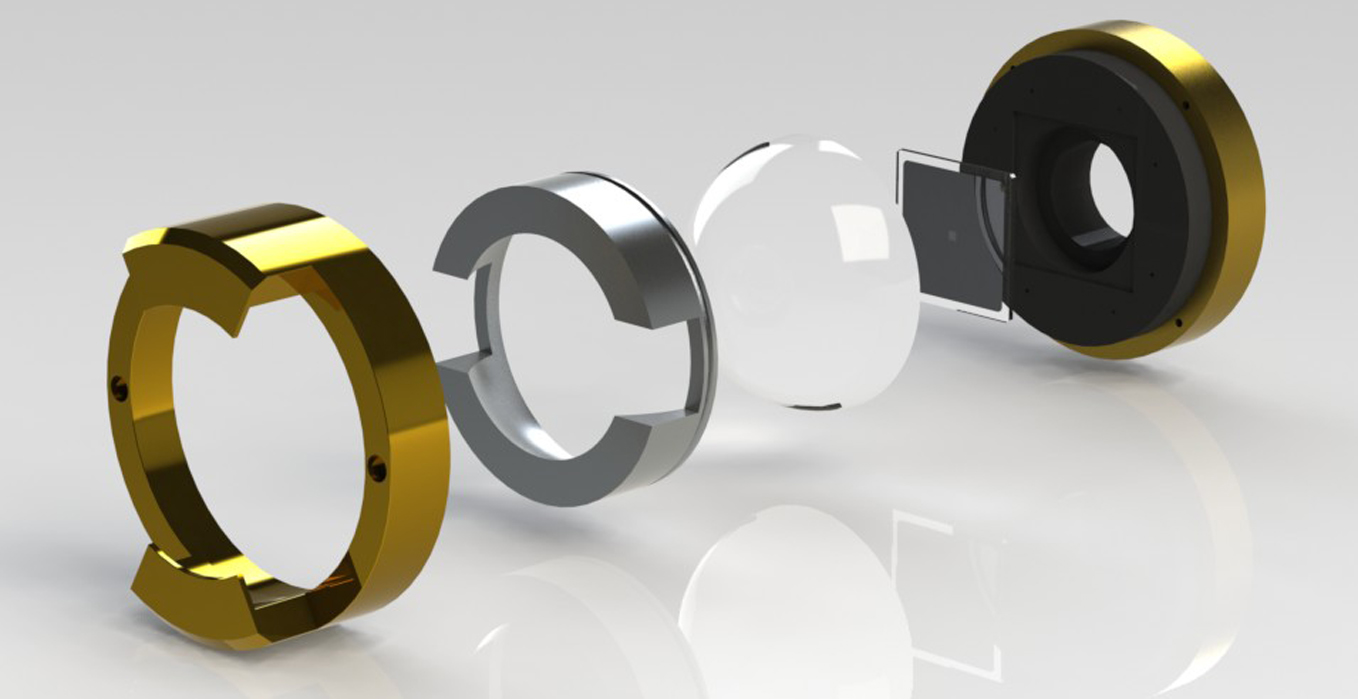
\includegraphics[width=\linewidth]{hemispherical-prism}
\caption{Exploded view of the sample mount for use with a hemispherical prism. The prism is adheared to the glass substrate using index matching fluid. The rig allows azimuthal rotation of the sample and prism.\label{fig:hemispherical-prism}}
\end{figure}
Some samples presented in this thesis are investigated so that the grating is embedded in a high-index substrate. For such samples, a hemispherical prism arrangement is used (figure \ref{fig:hemispherical-prism}). This allows illumination of the sample without the need for any corrections to the polar angle which might otherwise be necessary because of refraction. The sample is affixed to the prism using index-matching fluid.

\section{Scatterometry}
Scatterometry has been used previously to record the scattering patterns from samples found in Natural Photonics, such as the naturally diffuse scattering of the [name] beetle or the [name] butterfly. It has also been used to show the hexagonal shaped Brilloun zone of a pesdo-hexagonal lattice found in [this animal]. 

In this work, the previously reported experiential arrangement [ref] has been modified by the addition of spectral filters to limit the image accquired to a single wavelength. Using a plasmonic grating sample, the scatterometer directly images the equi-energy surface of the plasmonic dispersion. By applying a simple deformation to the aqquired image, the scatterometer provides a map of the coupled SPP equi-energy contours in momentum-space over the entier incident light cone. 
\subsection{Principle of Operation}
\begin{figure}
\centering %\documentclass[]{standalone}
%\usepackage{amsmath}
%\usepackage{amsfonts}
%\usepackage{amssymb}
%\usepackage{graphicx}
%\usepackage[table]{xcolor}
%\usepackage{auto-pst-pdf}%for converting pstricks diagrams for compilation in pdflatex
%\usepackage{pst-optexp} %for optics diagrams using pstricks
%\usepackage{wasysym} %for the sun symbol used for light source
%%\usepackage{subfig}
%%\usepackage[para,symbol*]{footmisc}
%\usepackage{tikz}
%%\usepackage{color}
%\usepackage{import}
%\usepackage{pst-solides3d}
%\usepackage{rotating}
%\usepackage{todonotes}
%\renewcommand{\arraystretch}{1.5}
%
%\begin{document}
\begin{pspicture}[](8,6) %start optics diagram (8x6) grid

\pnode(3,6){S1} %labeled nodes are the positions in the (8x6) grid
\pnode(3,5){L1}
\pnode(3,4){Pol}
\pnode(3,3){L2}
\pnode(3,2){P1}
\pnode(3,1){BS1}

\pnode(1,1){M1}
\pnode(1.521,1){Sample}
\pnode(5,1){L3}
\pnode(6,1){F1}
\pnode(7,1){L4}
\pnode(8,1){CCD}

%components in form \name[options](node1)(node1){label on diagram}

\lens[compname=L1,labeloffset=-1](S1)(Pol){L1}
\optplate[compname=Pol,labeloffset=-1](L1)(L2){Pol}
\lens[compname=L2,position=0.5,labeloffset=-1](Pol)(P1){L2}
\pinhole[compname=P1,phwidth=0.1,labeloffset=-1](L2)(BS1){P1}
\mirror[compname=BS1,bsstyle=plate,labelangle=-45](P1)(BS1)(M1){BS}
\mirror[compname=M1,mirrorradius=1,mirrortype=extended, mirrorwidth=1.7](BS1)(M1)(BS1){M1}
\pinhole[position=0.345,phwidth=0.1](BS1)(F1){P2}
\optplate[compname=Pol,labeloffset=-1,position=1.5](L3)(F1){Pol}
\mirror[compname=Sample,mirrortype=extended, mirrorwidth=0.25,labelangle=-80,labeloffset=1.1](M1)(Sample)(M1){G}
\lens[compname=L3,position=0.75,n=1.4](BS1)(F1){L3}
\optplate[compname=F1,position=0.7,optional](L3)(L4){F}
\lens[compname=L4,n=1.55](F1)(CCD){L4}
\optbox[compname=CCD,position=end,labeloffset=0,optboxwidth=1](L4)(CCD){CCD}

\psline{->}(5.75,1)(5.75,1.25)
\rput(5.75,1.45){$r$}
\psline[linestyle=dotted]{}(1,1)(1.521,1)
\rput(1.25,1.175){$\theta$}

\rput(S1){\Large{\sun}} %the sun symbol (not in opt-exp but nice anyways)


%add the beam, in the form \drawwidebeam[options](source){go through this node}{then this one}{then this one}

\addtopsstyle{Beam}{fillstyle=solid, fillcolor=green,opacity=0.05,linestyle}
\drawwidebeam[beamdiv=25, ArrowInside=->,arrowscale=1.3](S1){L1}{L2}{P1}{BS1}{M1}{Sample}{M1}{L3}{L4}{CCD}


\end{pspicture}
%\end{document}
\caption{scatterometer \label{fig:scatterometry}}
\end{figure}
A schematic of the scatterometry arrangement is shown in figure \ref{fig:scatterometry}. White light is directed through a collimating lens, L1 and an optional linear polariser allows the investigation of the polarization sensitivity of the acquired image.  The white light then is focussed through an alignment pinhole and the beam is reflected via the beam-splitter, BS, on to an ellipsoidal mirror with an eccentricity of 0.833. The mirror, M1, focusses the light onto the sample, positioned at G. 

If aligned precisely, the cone of light focussed by the mirror will include light from all directions (all azimuthal, $\phi$, angles) and a range of polar angle ranging from $\theta \approx 2^\circ$ to $\theta \approx 90^\circ$. The lower limit of $\theta$ being determined by the shadow cast by the sample itself. 

The reflected light from the sample is then collected by the same ellipsoidal mirror, M1 and is focussed through a second alignment pinhole, P2, positioned at the mirror's secondary focal point. This light is then collimated, passed through a spectral filter and imaged using a CCD camera. The acquired image is a directly mapped reflectivity plot of all polar and azimuthal angles, $R(\theta,\phi)$, with a high resolution determined by the pixel size and density of the CCD.
Using a range of spectral filters, the wavelength, and hence energy, of the map can be selected. The filters used are: $450\pm5$ nm, $500\pm5$ nm, $550\pm5$ nm, $580\pm5$ nm, $600\pm5$ nm, $650\pm5$ nm,  $700\pm5$ nm and $750\pm5$ nm. 

\subsection{Sample Preparation}
Since the lower limit of polar angle, $\theta$ is determined by the size of the sample area, a small sample area is desirable ot maximise out polar angle range. 
The grating samples are prepared by template stripping from a Si master, (a process detailed in Chapter \ref{}) to the center of a large plate of glass, which acts as the substrate. The grating is then further reduced in size by using a clean razor blade to remove excess sample area. 

Most previously reported work using scatterometry use a glass pippette to place the sample at the focal point of the ellipsoidal mirror, which casts a characteristic shadow which may hide important spatial features. By using a large glass plate substrate which covers the entirety of the the mirror face, shadows from alternative positioning devices are avoided. It is found, by comparison of our final images with calculated diffraction edges and theoretical predictions, that any distortion effects due to refraction through the substrate are negligible.


\subsection{Corrections and Momentum-Space deformation}
To obtain a map of momentum-space from the scatergrams, two image deformations are required. The first corrects the aberration of the ellipsoidal mirror to obtain an image whose radial axis is linearly scaled with respect to the polar angle, $\theta$. This correction is detailed in previous work \ref{}. 

The second deformation, scales the radial axis of the image to be proportional to the in-plane momentum, such that the reflectivity plot, $R(\theta, \phi)$ becomes,
\begin{align*}
R(\theta,\phi) \rightarrow R(k_0\sin\theta,\phi)\equiv R(k_x,k_y)
\end{align*}
Where $k_0 \sin \theta$ is the in-plane momentum for a specuallry reflected photon in the plane of incidence, at an azimuthal angle $\phi$. The effect of this deformation is illustrated in figure \ref{}. 
\begin{figure}
\centering 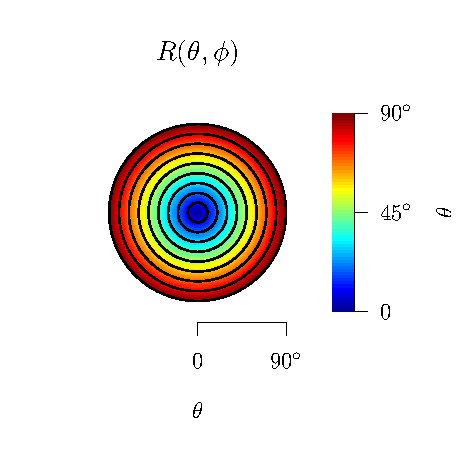
\includegraphics[width=0.5\linewidth]{figure-linear-theta-capsule}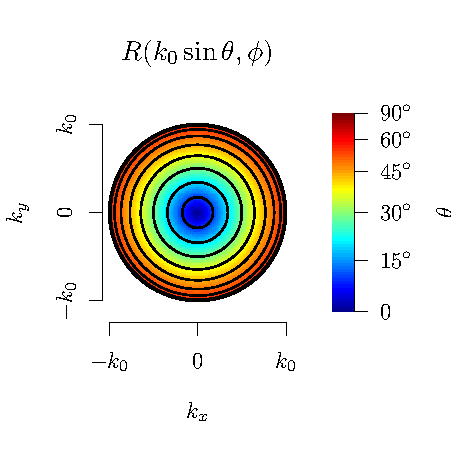
\includegraphics[width=0.5\linewidth]{figure-sin-theta-capsule}
\caption{The image deformation for $R(\theta,\phi) \rightarrow R(k_0\sin\theta,\phi)$. The black circles on both diagrams show contours of equal angle, ranging from $10^\circ$ to $90^\circ$ in $10^\circ$ steps.}
\end{figure}
This figure illustrates an important experimental consideration for the use of scatterometry for the direct imaging of momentum space. Due to the $\sin \theta$ radial dependence, at higher angles of $\theta$ the momentum space mapped provide less information the closer to grazing than at normal incidence. It is then possible to map a very large area of momentum space, while only illuminating up to $70^\circ-80^\circ$ degrees.
\subsection{Example dataset}


 

\end{document}
